\documentclass{school-22.211-notes}
\date{February 27, 2012}

\begin{document}
\maketitle

\topic{Temperature Effects on Cross Section (Doppler Broadening)}
\hi{Doppler Broadening} means, as the temperature increases, the width of the spectrum decreases, though the area under the curve stays the same. There are two possibilities: 
\begin{enumerate}
\item Infinite RI (infinite dilution factor) is independent of temperature becase the area under the psi chi curves are constant. 
\item Effective RI (finite concentration of \ce{^{238} U}) is dependent of temperature because of the self-shielding effect: as temperature increases, $\RI_{\eff}$ would increase. Also, as U/H increases, the fraction change of $\RI_{\eff}$ would increase as well as illustrated in Figure~\ref{Doppler}. That is, \textit{The higher the concentration of U238, the larger the Doppler temperature effects become.}
\end{enumerate}

In general, doppler broadening is the broadening of spectral lines due to the Doppler effect caused by a distribution of velocities of atoms or molecules. There are a couple of different kinds of Doppler broadening, including the thermal Doppler broadening due to the thermal motion of the particles; also, there are broadening depends on the frequency of the spectral line, the mass of the emitting particles, and the temperatures. 

Reference 1: Reuss Section 8.4. 

Reference 2: Handbook of Nuclear Engineering Chapter 4 Section 3. 

\begin{figure}
  \centering
  \subfloat[U/H=0.01]{\label{UH0.01}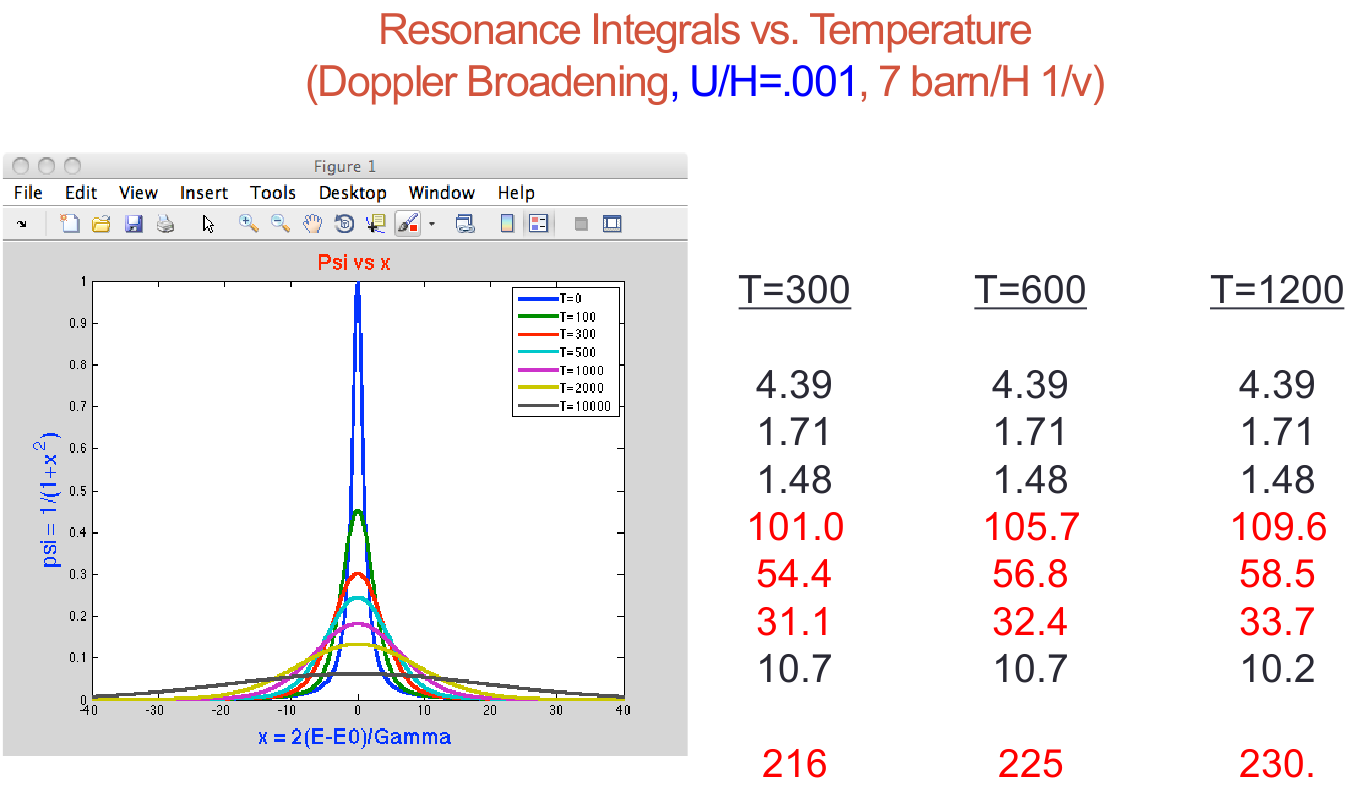
\includegraphics[width=0.5\textwidth]{images/Doppler-RI-1.png}}
  \subfloat[U/H=0.1]{\label{UH0.1}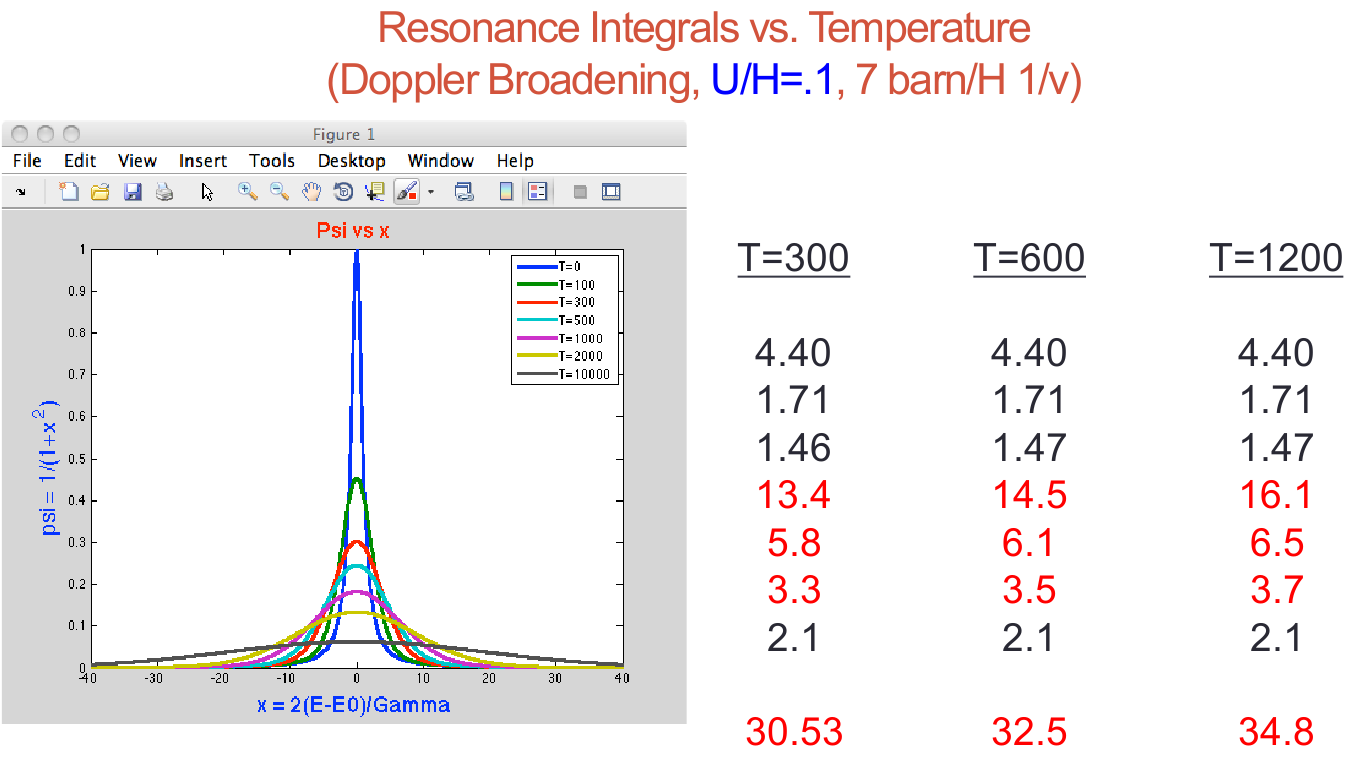
\includegraphics[width=0.5\textwidth]{images/Doppler-RI-2.png}}  
  \caption{Impact of Temperature On Effective RI/Resonance Absorption, Doppler Broadening} \label{Doppler}
\end{figure}

\topic{Energy Self-Shielding Effects}
As we increase the U/H ratio, the RI decreases in the three big resonance regions, and we see big dips on the spectrum plot. When U/H = 1.0, the spectrum is distorted. There are so much U238 in the fuel, that there is no flux in the fuel anymore. As we increase the number of uranium atoms by a factor of 10, the number of absorption per atom is decreased by a factor of 3. That is, the total aborption still increases, but the absorption per atom decreases. Figure~\ref{self-shielding} illustrates that RI are very dependent on the density of resonant materials. 

\begin{figure}
  \centering
  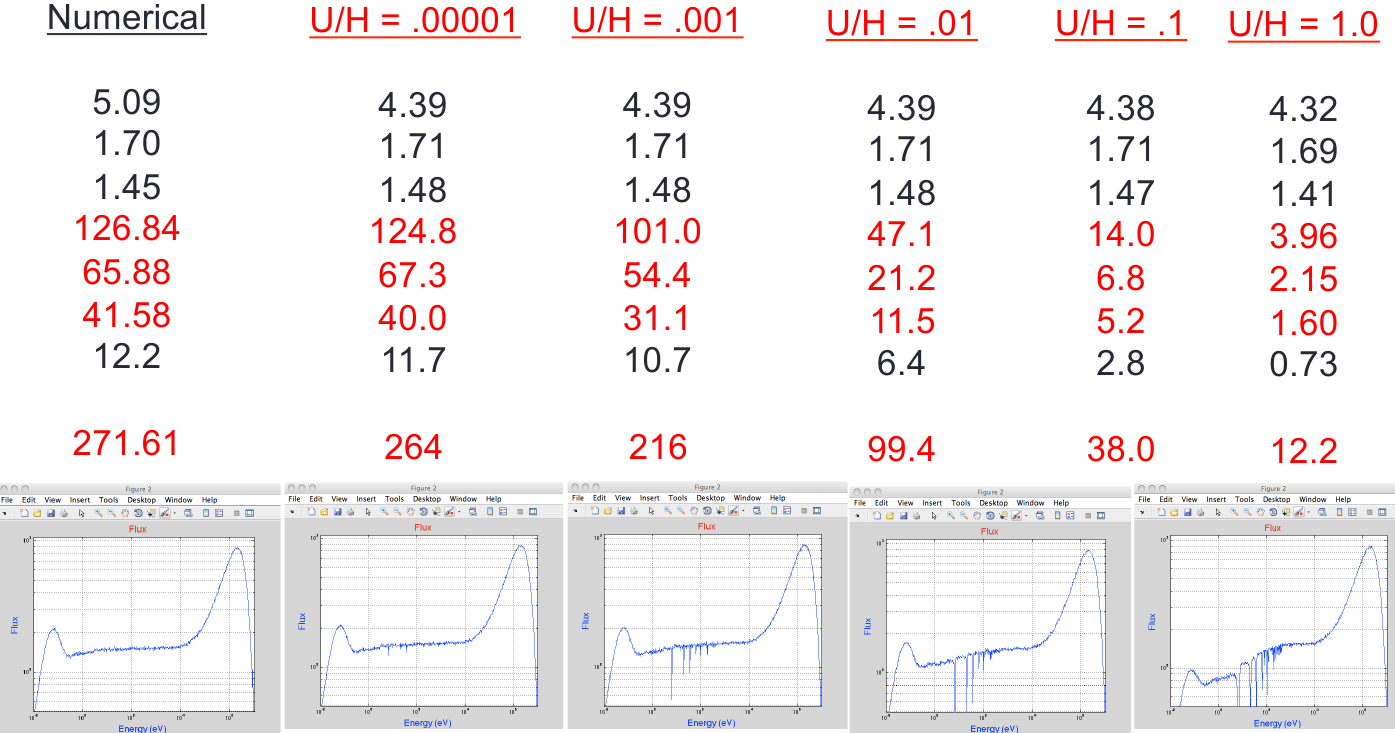
\includegraphics[width=4in]{images/self-shielding.png}
  \caption{Impact of Energy Self-Shielding On RI} \label{self-shielding}
\end{figure}

\topic{Spectral Hardening Shifts Resonant Absorption Rates}
\textit{As more absorber (uranium in this case) is added, the higher energy ranges become more important (more absorption happens in the higher energies), and the peak of the thermal spectrum shifts to the right.} Figure~\ref{spectral-hardening} also illustrates that self-shielding reduces the large resonance absorption fractions. 1/v absorption of U238 become more significant. 

\begin{figure}
  \centering
  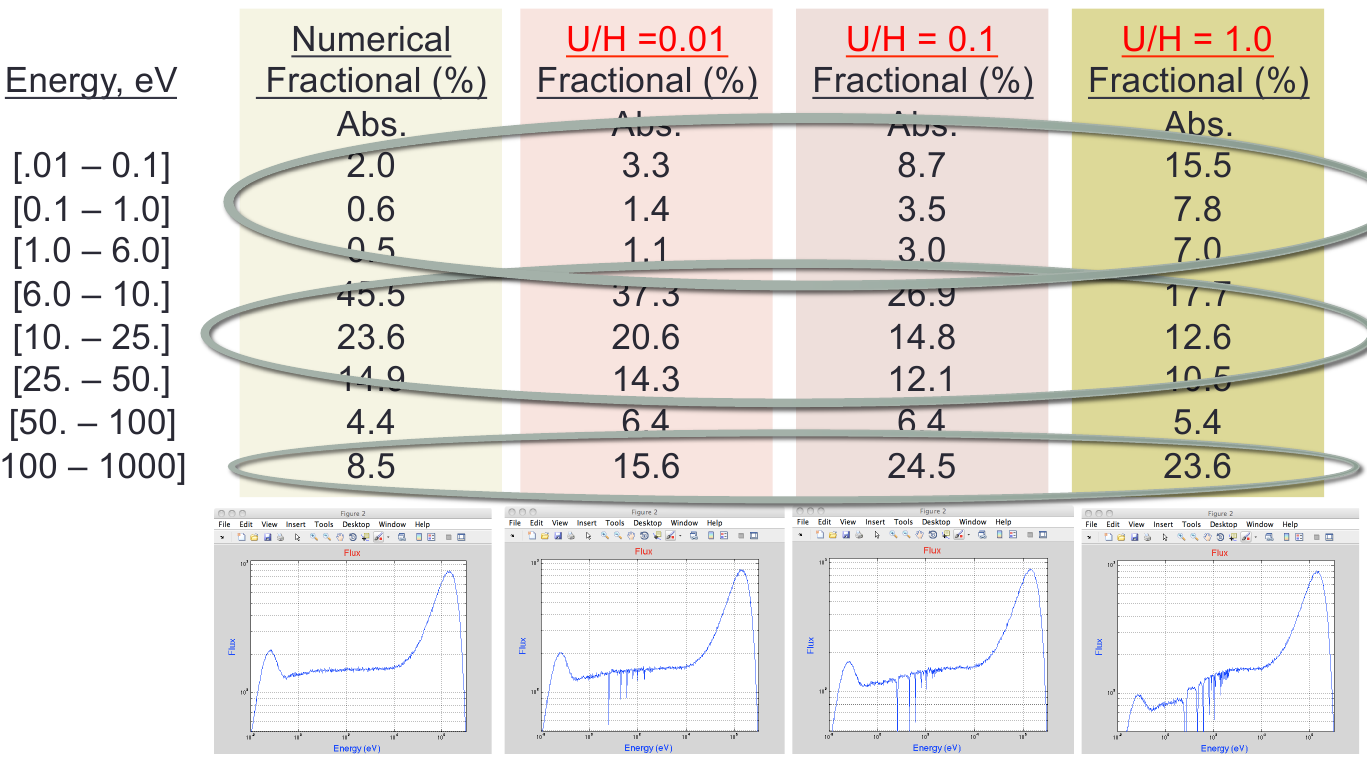
\includegraphics[width=4in]{images/spectral-hardening.png}
  \caption{Impact of Spectral Hardening On RI} \label{spectral-hardening}
\end{figure}

\topic{Reactor Type Spectral Optimizations and Sensitivities}

\topic{HW3: Slowing Down with Maxwellian Thermalization \& Resonance, Impacts of Self-shielding and Doppler}
HW3 adds U238 resonance model to our slowing down MC code. Notice only absorption resonance from 0 to 1 keV is considered for now. The result should look like Figure~\ref{HW3-result}. 

We should get column 1 and 4 in Lec 6,  slide 21. 

\begin{figure}
  \centering
  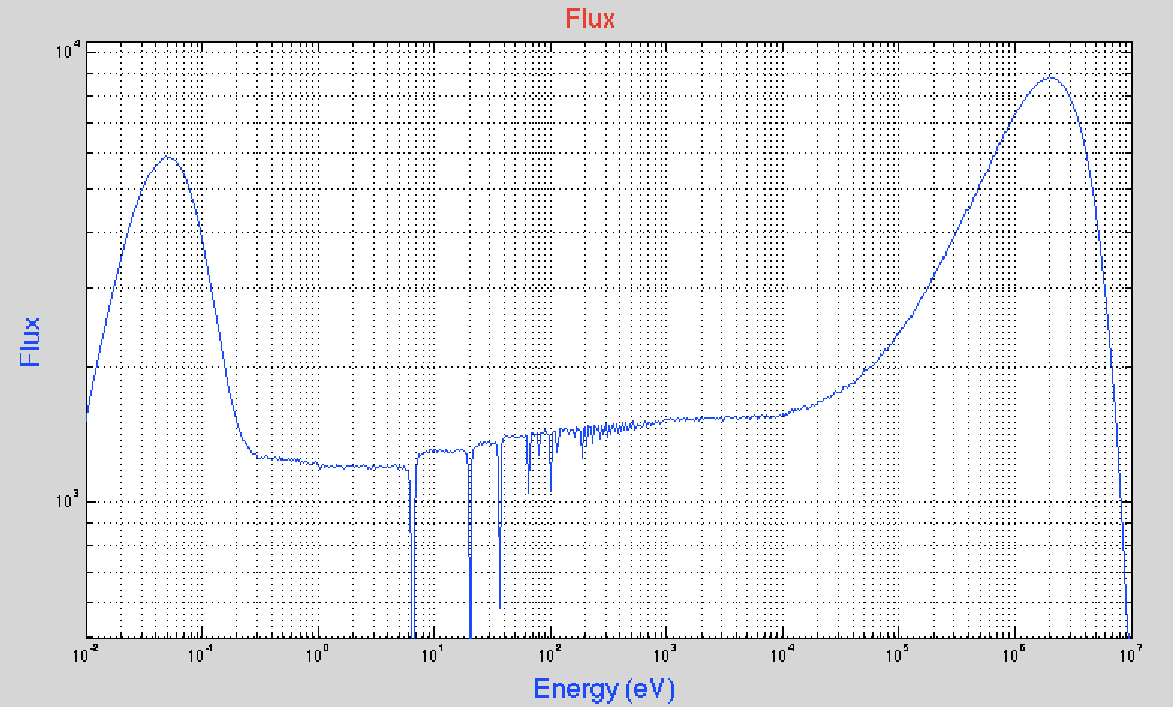
\includegraphics[width=4in]{images/HW3-result.png}
  \caption{Expected Plot From HW3} \label{HW3-result}
\end{figure}

\begin{figure}
  \centering
  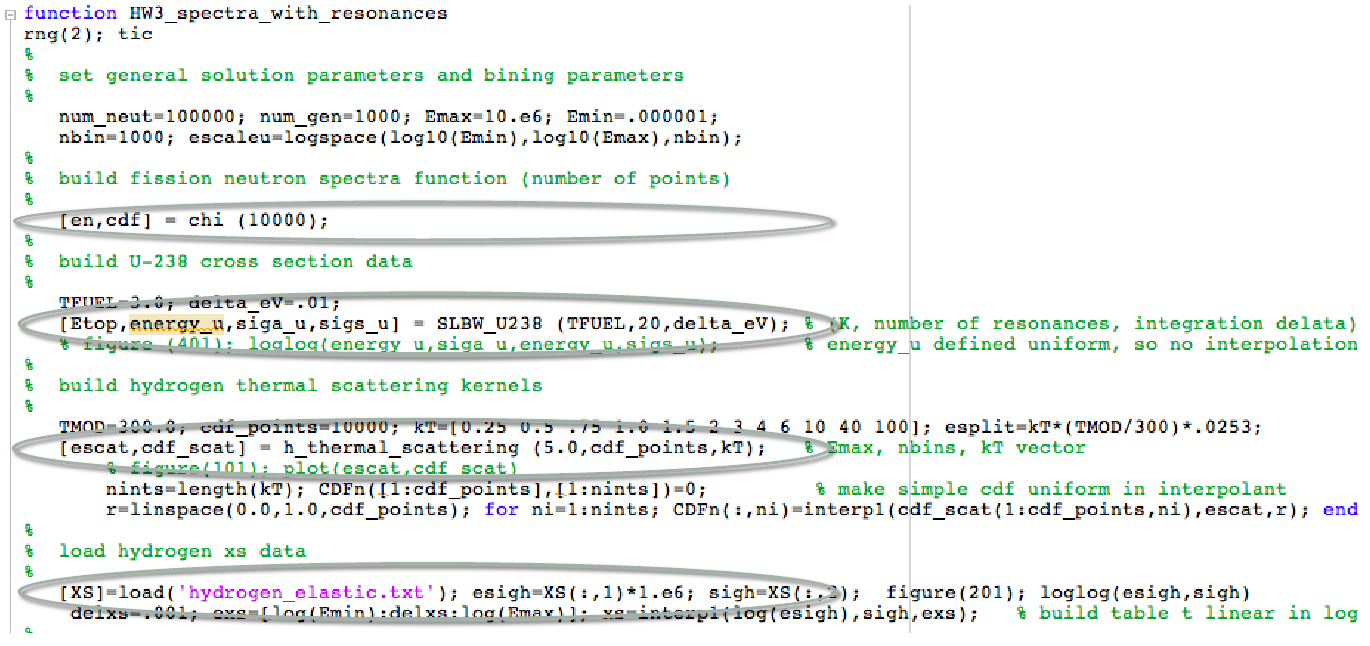
\includegraphics[width=4in]{images/spectral-code-11.png}
  \\
  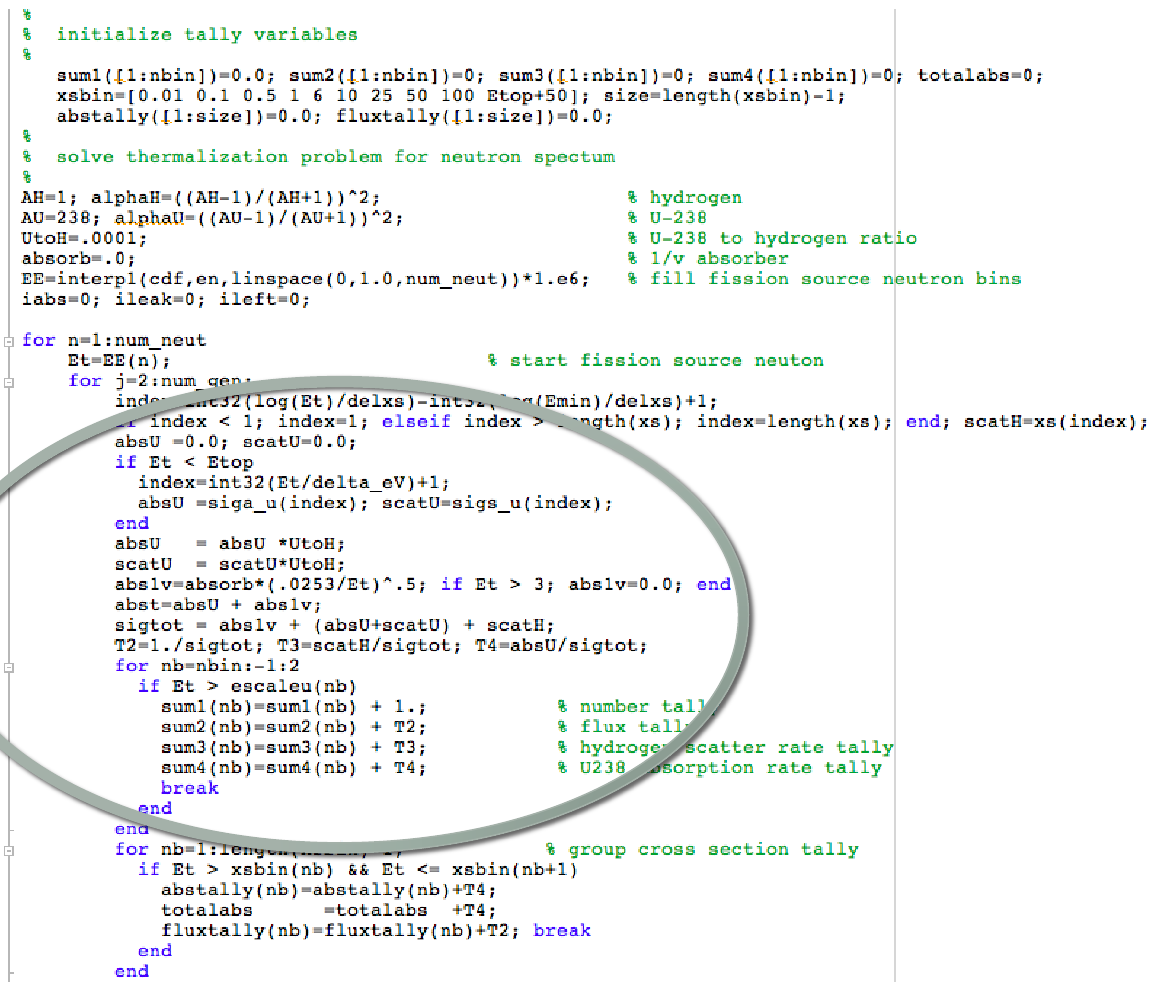
\includegraphics[width=4in]{images/spectral-code-12.png}
  \\
  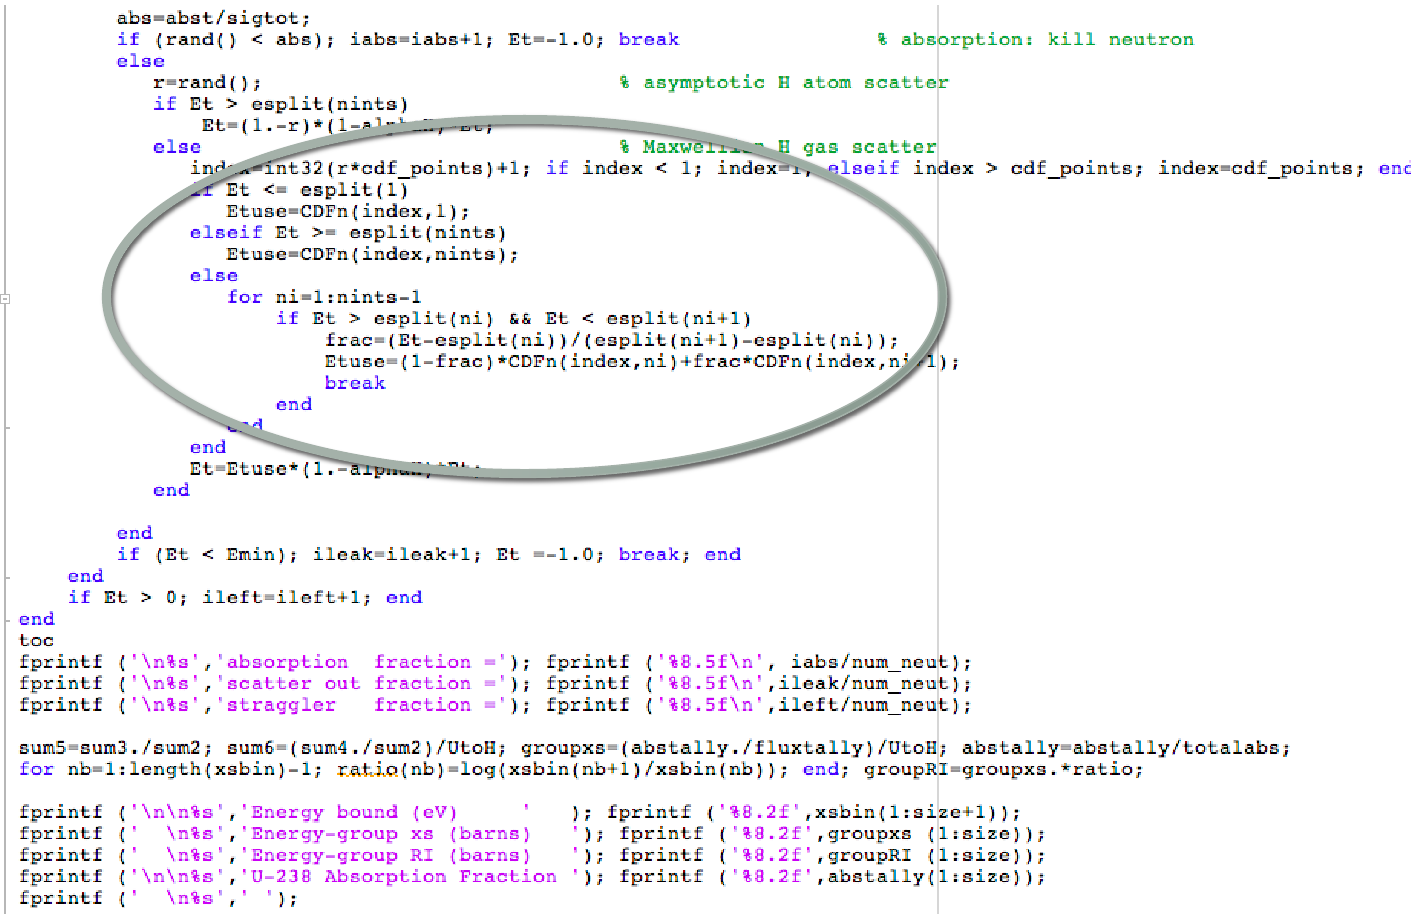
\includegraphics[width=4in]{images/spectral-code-13.png}
  \caption{Spectral Code With Resonance For HW3}
\end{figure}

\end{document}
